\chapter{Sistemas de Detecção de Queda}
\label{cap:sistemasRecomendacao}

Um \ac{FDS}, pode ser descrito com um dispositivo de apoio, cujo principal objetivo é alertar o usuário em um evento de queda \citep{igual2013challenges}. De forma geral, estes sistemas são capazes de distinguir \ac{ADL}  de um evento de queda. Este tipo de sistema pode ser desenvolvido de diversas formas é pode está tanto embarcado em um Dispositivo vestíveis como um smartwatch ou se basear em um sistema de monitoramento utilizando câmeras. 

Com o uso de sistemas de detecção de quedas é possível que o usuário tenha o seu medo de cair reduzido, e dependendo da solução que foi desenvolvida, possa ser socorrido de maneira muito mais rápida, caso necessário. Um individuo que que já sofreu uma queda, pode desenvolver uma sindrome chamada \ac{FOF}, que pode levar a perda da capacidade de se realizar atividades rotinieiras, como passear em um parque, ou assistir um filme em família \citep{legters2002fear}.

As seções desse capítulo são organizadas da seguinte maneira: A seção \ref{sec:fall_definition} define o conceito de quedas e expõe os diversos estados da mesma; A \ref{sec:fall_system_types} irá demonstrar os 3 diferentes tipos de sistemas de detecção quedas mais populares; A seção \ref{sec:sensors} irá demonstrar os principais sensores utilizados nos sistemas de detecção de quedas; Por fim, a seção \ref{sec:fds_examples}  irá mostrar exemplos de aplicações que realizam a detecção de quedas. 



\section{Definição de Queda}
\label{sec:fall_definition}
De forma geral, podemos definir uma queda como um evento súbito e involuntário, onde o indivíduo de uma posição em pé ou sentado, passa a ocupar uma posição integral ou parcialmente deitada (Horizontal). Na busca por uma definição mais formal, em 1987, o Kellog International Working Group on the prevention of falls, descreveu uma queda como "Vir ao chão ou algum nível mais baixo, sem a intenção como consequência de um golpe violento, perda de consciência, ou início súbito de paralisia como no caso de um acidente vascular cerebral ou um ataque epiléptico"  \citep{igual2013challenges}. Quando analisamos uma queda através das pesperctiva da aceleração do movimento, ela pode ser dividida em etapas descritas na imagem \ref{fig:fall_states}. Estas 4 etapas são as seguintes:


\begin{figure}[ht]
	\centering
	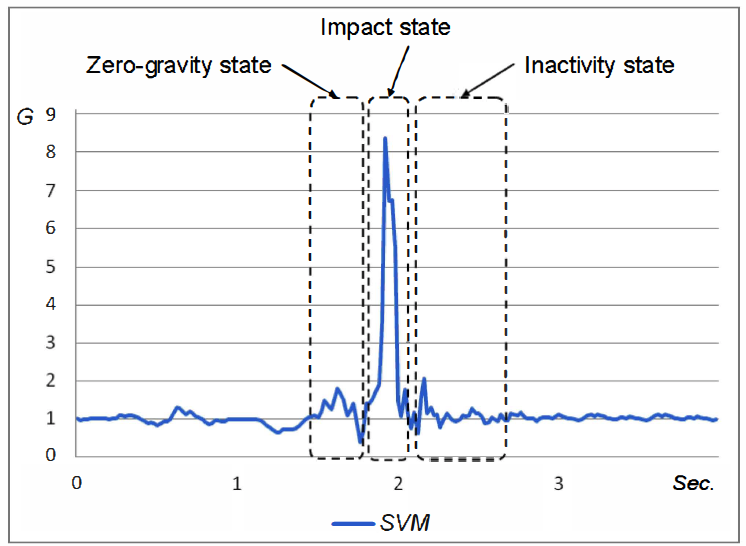
\includegraphics[width=.8\textwidth]{imagens/fall_states.png}
	\caption{Etapas de uma queda \citep{hsieh2014wrist}.}
	\label{fig:fall_states}
\end{figure} 


\begin{itemize}
	\item{\textbf{Período Anterior a Queda (Pre-Fall)}: Durante este período o individuo estará realizando suas atividades cotidianas, que podem levar ou não a um pico de aceleração que deve ser tratado para que se possa evitar falso-positivos. Ações que geralmente levam a este pico de aceleração são movimentos como sentar ou se deitar muito rápido, ou dependendo da posicionamento dos sensores, atividades físicas que exigem bastante movimentação. }
	
	\item{\textbf{Período Anterior a Queda (Pre-Fall)}: Durante este período o individuo estará realizando suas atividades cotidianas, que podem levar ou não a um pico de aceleração que deve ser tratado para que se possa evitar falso-positivos. }
	
	\item{\textbf{Período Queda Livre (Free-Fall)}: Durante este período o individuo está se descolando em direção ao chão. Nesta fase o valor de sua aceleração irá tender a 0.  }
	
	\item{\textbf{Período do Impacto (Impact-Phase)}: Período caracterizado pelo impacto do índividuo, este período é crítico na aplicação, poís é onde ocorre o pico de aceleração. }
	
	\item{\textbf{Período de Inatividade (Inactive State)}: Período posterior a queda, onde o usuário irá realizar o esforço para se levantar. Em quedas mais graves, onde o usuário está incapaz de se movimentar ou inconsciente este valor se modificação de maneira muito sutil, porém de forma geral, o usuário que sofreu uma queda não se levanta imediatamente. De acordo com \cite{mehner2013location}, o período de pós impacto e inatividade levá aproximadamente 2 segundos.  }
	
\end{itemize}


\section{Tipos de Sistemas de Detecção de Queda}
\label{sec:fall_system_types}
Diversos tipos de Sistemas de Detecção de Queda foram desenvolvidos nos últimos anos e estes utilizam diferentes abordagens buscando atingir o mesmo objetivo: realizar a detecção automática das quedas. De acordo com \cite{mubashir2013survey}, estes sistemas podem ser categorizados em três grupos: sistemas de detecção baseados no ambiente, sistemas de detecção baseados na visão, sistemas de detecção baseados em tecnologias vestíveis.

\subsection{Sistemas de Detecção Baseados no Ambiente}
Sistemas de detecção baseados no Ambiente utilizam a fusão de dados obtidos de diversos sensores para realizar a detecção de quedas. Atravês desses sensores são obtidos sinais audio-visuais e dados vibracionais do ambiente que está sendo monitorado. Este tipo de sistema podem ser divididos em duas categorias:

\begin{itemize}
	\item{\textbf{Audio-Visuais}: Neste tipo de sistema são analisados os sinais audio-visuais obtidos atravês de câmeras e microfones espalhados no ambiente desejado. Um exemplo deste sistema foi proposto por \cite{zhuang2009acoustic}, ele utiliza o padrão da onda sonora capturada, com uma base de dados treinada  com diferentes tipos de onda sonoras associadas com diferentes tipos de eventos. Sendo assim, capaz de diferenciar uma queda de uma atividade diária. }
	
	\item{\textbf{Dados Vibracionais}: Neste tipo de sistema são analisados os dados vibracionais obtidos atravês de sensores de vibração espalhados no chão do ambiente desejado. Um exemplo deste sistema foi proposto por \cite{zhuang2009acoustic}, ele utiliza o padrão da onda sonora capturada, com uma base de dados treinada  com diferentes tipos de onda sonoras associadas com diferentes tipos de eventos. Sendo assim, capaz de diferenciar uma queda de uma atividade diária. }
\end{itemize}



\subsection{Sistemas de Detecção Baseados na Visão}
Sistemas de detecção baseados na visão utilizam uma ou mais câmeras posicionadas ao redor do ambiente desejado para  que se possa realizar a detecção de quedas. As camêras são consideradas um meio menos intrusivo de detecção, pois, diferente dos sistemas que utilizam tecnologias vestíveis, somente o video gerado pela câmera são utilizadas na detecção, sem a necessidade do usuário vestir nenhum dispositivo eletrônico. Diferentes tipos de técnicas de processamento de video e imagem são utilizadas na detecção. As principais delas são:  

\begin{itemize}
	\item{\textbf{Espaço-Temporais}: Sistemas que utilizam caracteristicas espaço-temporais para realizar modelagens capazes de fornecer dados cruciais na detecção de diferentes tipos de atividades.  Um sistema proposto por \cite{foroughi2008eigenspace} realiza a extração de informações de movimento de uma sequência de video. Aplicando uma técnica chamada Eigenspace sobre as informações de movimento coletadas, é possível extrair um vetor de caracteristicas, que  é utilizado por um algoritmo de inteligência artificial, mais especificamente um algoritmo de redes neurais, para determinar o tipo de evento ocorrido. }
	
	\item{\textbf{Inatividade/Mudança de Forma}: Sistemas que utilizam mudanças de forma e ausência de atividade no monitoramento em video para realizar a detecção de quedas. Um exemplo deste tipo de sistema foi proposto por \cite{rougier2011robust}. Em seu artigo, são utilizadas técnicas de detecção e análise de formas para detectar a silhueta e atividade (representado por mudanças de forma) do indíviduo que está sendo monitorado. Para que se possa diferenciar quedas das atividades diárias, é utilizado o método de \textit{Mistura de Modelos Gaussianos}, um método estastístico utilizado em visão computacional.}
	
	\item{\textbf{Postura}: Sistemas que identificam e localizam diversas posturas do individuo, calculadas através das diferentes posições corporais, utilizando uma sequência de imagens para realizar a detecção um evento de queda. \cite{cucchiara2005probabilistic}, desenvolveu um sistema de detecção que analisa os histogramas das imagens geradas pelas câmeras, para classificar as posturas do individuo monitorado e consequentemente detectar um evento de queda.  }
	
	\item{\textbf{Análise 3D da Posição da Cabeça}: Sistemas que realizam o monitoramento da cabeça do individuo, e atravês de modelos de estado é capaz de detectar as magnitudes do movimento realizado. Um exemplo deste tipo de sistema foi proposto por \cite{rougier2005demo}, ele realiza a modelagem 3D da cabeça do individuo e capaz de calcular a velocidade e a trajetória deste modelo que são posteriormente utilizadas na categorização do evento como queda.}	
\end{itemize}



\subsection{Sistemas de Detecção Baseados em Tecnologias Vestíveis}
Sistemas vestíveis de detecção de quedas utilizam os dados de sensores que estão acoplados sobre ou na roupa dos usuários. Este tipo de sistema apresentam claras vantagens sobre tanto os sistemas baseados no ambiente ou na visão. Ambos os tipos de sistema, exigem um custo constante de manuntenção, que dependendo de como o sistema foi desenvolvido, pode ser bastante alto, além disso a área de atuação do sistema fica limitada a uma área pré-determinada (e.g quarto, sala de estar). Utilizando tecnologias véstiveis não temos este problema, pois o usuário poderá leva o seu dispositivo para onde ele desejar.

Levando em consideração a privacidade do usuário, os sistemas vestíveis levam vantagem em relação aos baseados no ambiente e na visão. A necessidade de uma monitoração por vídeo constante necessária em alguns desses sistemas podem deixar o usuário relutante em implementar está solução. 

De acordo com \cite{igual2013challenges}, o uso de smartphones para realizar a detecção de quedas tem sido uma tendência devido ao seu baixo preço, altos volumes de produção e facilidade de desenvolvimento. O grande problema do uso do smartphone é justamente o seu posicionamento. O aparelho pode estar em diversas posições, ou mesmo, nem diretamente ligado ao corpo do usuário. Está incerteza dificulta bastante o uso deste tipo de dispositivo no reconhecimento de atividades. 

Tentando resolver este problema, o uso de aparelhos realmente vestíveis vem sendo utilizado em sistemas de detecção de quedas, como pode ser visto nos trabalhos desenvolvidos por \cite{hsieh2014wrist} e \cite{pivato2011wearable}.


